
\section{Spatial Distribution of Cities and Violence}
\label{theory}

The extant literature has made important strides in explaining the relationship between economic growth and civil conflict. Yet, none to our knowledge have explored the effects of subnational overlaps in the spatial distribution of cities and conflicts. We argue that this overlap is key to explaining variation in macroeconomic performance during civil conflict. 

Our argument on the proximity of conflict to cities should not be confused with arguments focusing on simply the area covered by a conflict. Our argument explicitly differs in the hypothesized mechanism through which conflict affects economic performance. We do not disagree that the spread of a conflict could impact state economic prospects, but we argue that a large conflict area is not a necessary condition for poor economic performance. Conflict area is only one possible proxy for overall destructiveness. However, conflicts with smaller spatial areas can be similarly disruptive if they are centered near urban centers. In fact, we anticipate measures of conflict proximity relative to cities rather than spread to be more appropriate to test the macroeconomic effects of conflict.

\subsection{Cities and Economic Growth}

That cities are central to national economic performance is well supported in the relevant literature. \citet{myrdal:sitohang:1957} were among the first to argue that once cities reach a certain size through the process of urbanization, they tend to become self-reinforcing growth centers through a process Myrdal termed as ``cumulative causation''. \citet{chenery:syrquin:1975} provided support for this idea by showing that sharp declines in fertility and substantial increases in growth per capita typically follow cases of urbanization. Jane Jacobs, a progenitor of the move towards focusing on urban centers, went farther than most in her time by arguing that cities are the primary motivators of state economies and should be given primacy over the nation state in economic analysis \citep{jacobs:1969,jacobs:1984}. 

In the past three decades, as the pace of urbanization has accelerated, economists have devoted even more energy to investigating the role of city-level economic drivers \citep{lucas:1988, ciccone:hall:1996, begg:1999, henderson:wang:2007}. Most notably \citeauthor{krugman:1991a}, in his seminal 1991 article, ``Increasing Returns and Economic Geography'', convincingly showed the importance of studying economic outcomes within a spatial context. A key finding of Krugman's work on economic geography has been the importance of agglomeration effects, the idea that ``activities tend to cluster where markets are large and markets become larger where activities cluster'' \citep{krugman:1997}. \citet{henderson:2000} provides empirical evidence for why these agglomeration effects would manifest by showing that spatial clustering promotes economic efficiency in a variety of ways from simply enabling savings in transport costs to producing more efficiently functioning labor markets.

In addition to agglomeration effects, there is an even simpler story, which can be traced back to \citet{marshall:1920}, that states geographic clustering of firms promotes valuable learning and exchange between actors. \citet{lucas:1988} provides a formal treatment of this argument and shows that the accumulation of human capital generates positive spillovers, where if even one worker acquires a new skill then spatially proximate workers would all become more productive. Empirical estimates of agglomeration effects indicate that a doubling of employment density corresponds to a 5\% increase in labor productivity \citep{ciccone:hall:1996,ciccone:2002}. \citet{glaeser:etal:1992} examine this problem empirically and show that cities are important for economic growth precisely because they lead to the knowledge spillovers that are important for innovation. Similar empirical results have been found by many others and have led to a growing consensus that cities can serve as important knowledge hubs for national economies \citep{jaffe:etal:1993, glaeser:1994, firestone:2010}. 

% Further \citet{quigley:1998} concludes that ``large cities have been and will continue to be an important source of economic growth.'' good quote but i didnt know where to put it

\subsection{Cities and Conflict}

The econometric evidence on the importance of cities has crucial implications for our understanding of the spatial structure of subnational economies. Specifically, at the subnational level, the economy can be thought of as consisting of ``lumps'' of productivity and swaths of areas that contribute little to macroeconomic growth \citep{venables:2005}. This implies that subnational conflicts will have heterogeneous effects on economic growth given their spatial proximity to economically relevant centers such as cities.

\citet{glaeser:shapiro:2002} discuss the historic role of cities in warfare and their current role with respect to terrorism. Cities, they argue, once provided safe haven in the midst of conflict; defense of a concentrated population is easier than defense of a dispersed population. However, as the tactics of warfare have shifted over the centuries, the relationship between violent conflict and cities has become more complex. Dense populations also tempt belligerents and maximize the impact to cost ratio of a given violent action. 

Additionally, warfare destroys transportation infrastructure, which can interfere both with commerce and with rebuilding during a conflict. In particular, conflict affects a citizen's ability and willingness to participate in commerce. When major population centers are threatened by violence, residents will be less likely to engage in economically productive activities. Violence near major population centers not only threatens residents directly, but impedes business by threatening trade between the population center and other cities or rural areas. 

We extend this line of research by conceptualizing civil war not as a homogeneous national phenomenon, but as a diverse class of violent conflict with properties that distinguish the effects of one conflict from another. Since urban economies are responsible for a disproportionate share of national economic performance, civil conflicts in or near these engines of commerce should likewise exert a disproportionate influence on state performance. 

\subsection{Descriptive Cases}

This hypothesis does not seem unknown to armed actors. The guerilla group Fuerzas Armadas Revolucionarios de Colombia (FARC) appears to have internalized these mechanisms. In 1998 and 1999, the organization moved its violent operations from mostly rural areas of Colombia into major cities and near to the capital (Petras and Brescia 2000). This coincided with economic strain caused by the implementation of an IMF/World Bank structural readjustment program. However, the timing was likely not coincidental. FARC advocates a number of political and economic reforms and chooses targets strategically related to these objectives. Figure \ref{fig:columbiaMap} shows the spatial distribution of violence in Colombia from 1989 to 2008, where Bogot\'{a} is designated by a black diamond and major cities by black triangles. To determine the centroid locations of conflict we use the PRIO conflict site database developed by \citet{hallberg:2012}. 

\begin{figure}[ht]
	\centering
	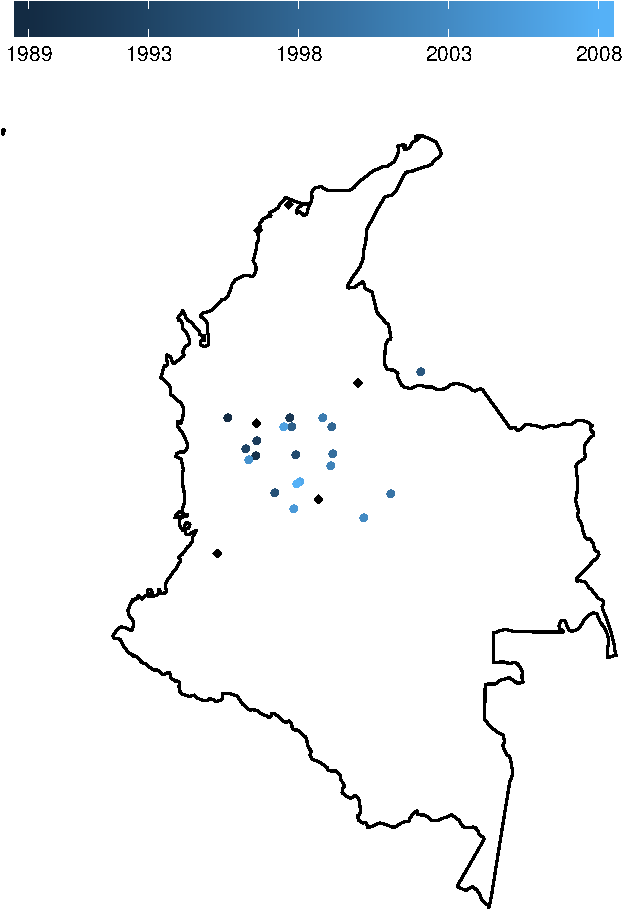
\includegraphics[width=.5\textwidth]{colombiaMap-crop}
	\caption{This map illustrates the geographic distribution of all conflict centroids in Colombia, according to the PRIO Conflict Site Dataset, and major cities from 1989 to 2008.}
	\label{fig:columbiaMap}
\end{figure}

Forbes magazine, reporting on peace talks between FARC guerillas and the Colombian government in 2012, wrote: 

\begin{quote}
	FARC's strategy and [beliefs have] always been to make economic pressure on both, multinational companies and the Colombian government. This has been done by attacking oil and natural gas infrastructure affecting companies such as Pacific Rubiales Energy, Oxy and Ecopetrol. For non-fuel related international companies with subsidiaries in Colombia, such as Goodyear, Nestle, Microsoft, Toyota, among others, FARC’s modus operandi was mainly racketeering, kidnappings and extortion. (Flannery 2012)
\end{quote}

By targeting economic centers and resource infrastructure, FARC can strain Colombia's economy, frighten investors, and bolster support from poor and rural workers sensitive to wealth disparity in the country. \citet{rabasa:chalk:2001} identify a three-pronged strategy pursued by FARC in the 1990s: to consolidate power in coca-growing regions, to conduct military operations in economically valuable areas, and to isolate major cities from the rest of the country by limiting communication and travel between them.  

More recently, economic productivity in Syria has ground to a halt due to its ongoing civil war. Fighting in Syria has been widespread with particularly bloody battles of attrition fought over some of the country's largest cities. Both Aleppo and Damascus have been divided neighborhood-by-neighborhood by the Assad regime and various armed groups vying for control of the cities. Simultaneously, Syria's economy has shrunk dramatically.

While FARC seems to exploit its ability to target areas of economic importance including cities, other insurgencies tend to be more peripheral. India, for instance, has faced challenges by armed groups in its north-east for half a century. However, this area of India is remote, primarily agrarian, and relatively less populous than other parts of India. Indeed, for much of this period, India has experienced relatively robust economic growth. In figure \ref{fig:indiaMap}, we show the geographic distribution of conflict in India from 1989 to 2007 again using the PRIO conflict site database. The story from this map is clearly quite stark from that of Colombia. Whereas in Colombia conflict had come right to the gates of major cities, in India conflict has been primarily confined to the periphery.

\begin{figure}[ht]
	\centering
	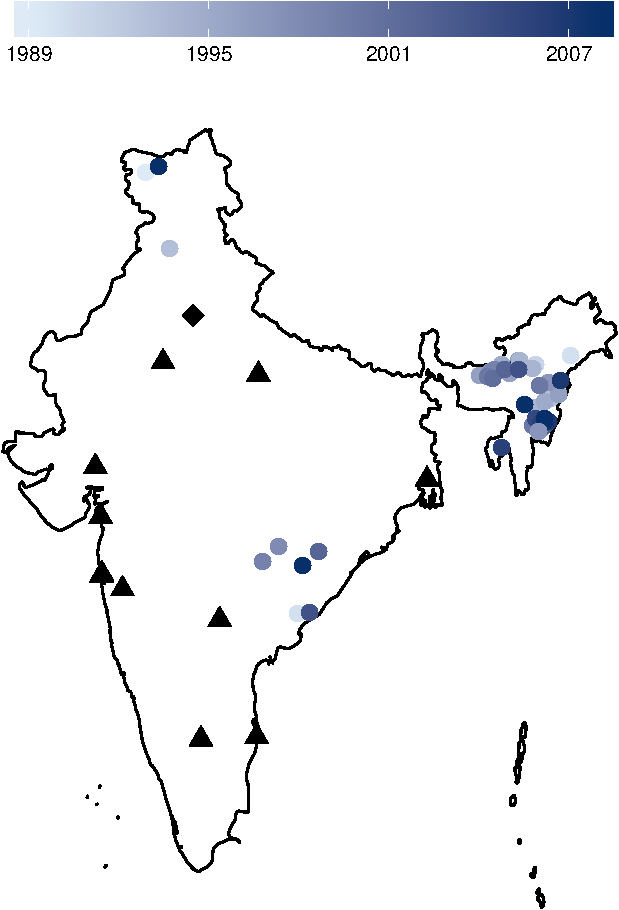
\includegraphics[width=.5\textwidth]{indiaMap-crop}
	\caption{This map illustrates the geographic distribution of all conflict centroids in India, according to the PRIO Conflict Site Dataset, and major cities from 1989 to 2007. }
	\label{fig:indiaMap}
\end{figure}

Nigeria and Cameroon have battled Boko Haram in a bloody conflict in their rural northern regions for half a decade. For the period between 2009 and 2013, the National Consortium for the Study of Terrorism and Responses to Terrorism (START) described Boko Haram as ``among the deadliest [terrorist groups] in the world'' \citep{pate:etal:2014}. The group's tactics range from car and suicide bombings to direct assaults to mass kidnappings. Nonetheless, Nigeria and Cameroon have both maintained strong economic growth during this period. The African Development Bank Group (AFDB) described Nigeria's economic growth from 2004 to 2014 as ``robust'' and projected ``moderate'' growth of 5\% for 2015 \citep{afdb:nigeria:2015}. On Cameroon, the AFDB said ``despite the security and humanitarian crisis in the region, Cameroonian growth remains strong at above 5\%'' \citep{afdb:cameroon:2015}.

It is important to note that Mexico does not appear in the civil war dataset chosen for this study. The UCDP definition of civil war requires that the conflict be fought over an ``incompatibility that concerns government and/or territory,'' a criteria not strictly met by the organized crime violence experienced by the country \citep[p.1]{themner:2014}. Nonetheless, we want to reiterate that this instance of armed conflict, of the magnitude typically associated with civil war, conforms to the expectations of our theory. Mexico, now nearly a decade into a violent and complicated conflict between several organized criminal enterprises and the federal government, has maintained healthy economic performance. For much of this time, the cartel violence generally occurred in rural areas along drug trafficking routes and not within major cities. \citet{beittel:2011} writes that ``drug trafficking-related killings remain concentrated in a relatively few cities.'' Meanwhile, several majors cities including the capital, Mexico City, have experienced relatively low levels of cartel violence.

The examples cited here seemingly break from the mold by prospering economically while facing high levels of internal violence. A common characteristic of these cases is the geographic distribution of conflict; violent armed groups operate primarily in rural areas away from major cities.
